\chapter{The Sensory Afferent Database}\label{ch:database}
\graphicspath{{D:/Github/Bipedal_Robot/Documentation/Reports and Papers/Dissertation/Figures/50-database/}{figs/50-database/}}

\section{The Database and What It Contains}\label{sec:sadb_resource}

The Sensory Afferent Database (SADb) gathers into one searchable resource the physiological specification from which the synthetic nervous system of Chapter~\ref{ch:sns} is assembled: what each class of Ia, Ib, and II afferent encodes, over what ranges of length, velocity, and force it operates, which interneuron populations it contacts, whether the action is excitatory or inhibitory, ipsilateral, contralateral, or both, and in which phase of the step cycle the pathway is open. That specification was established experimentally, one pathway and one preparation at a time, across a century of work in cat, mouse, rat, and human preparations, and much of it remains unknown or contested outside the pathway-rich core, scattered over an enormous primary literature. A controller designer, an animal researcher planning the next experiment, and a roboticist choosing what a sensor should imitate ask different questions of that same literature, and it answers none of them without being gathered, structured, and searchable first.

I built it within the AARL's NeuroNex Communication, Coordination, and Control in Nervous Systems (C3NS) effort and presented it at Neuroscience 2023 \citep{bolen_sensory_2023}, and later presented the AI-assisted triage study that expanded it at Neuroscience 2024 \citep{bolen_using_2024}. Its content is organized as five linked tables (Papers, Feedback, Models, Review Papers, and Recorders), with the DOI as the unique identifier wherever a record carries one. The Papers table is the core: each paper carries structured curation notes, one to three sentences of distilled mechanism written from the paper's own text, never from memory, with free-text fields constrained by controlled vocabularies for animal preparations and afferent classes. Each sensory feedback pathway is a record in its own right in the Feedback table, named by a fixed grammar of afferent, action, side, joint, and phase (for example, ``Ib stance to swing''), so that pathway records compose into circuits the way a controller will use them, and each is linked to the papers that established it. The Models table links each computational model of afferent control to its source paper and to the pathway records it implements, and the Review Papers and Recorders tables carry the review literature and the instrumentation papers behind the electrophysiology.

The database answers queries that no bibliography can. A designer can filter the corpus by afferent class, animal preparation, or pathway; follow a pathway record to the papers that established it in each species; walk the citation neighborhood of a candidate anchor paper; or count the corpus along any two dimensions at once. The database's primary form is the packaged explorer: a single-file, offline application embedding the full audited corpus, its citation graph, and its named topic clusters, with searchable and pivotable tables, focus-mode citation neighborhoods drawn in the laboratory's own convention of papers as neurons, and a generated knowledge base with cluster, pathway, afferent, and animal pages, running in a browser on any machine with no network connection (an off-the-shelf bibliometric viewer was tried first and retired within weeks: no drill-through from a cluster to its papers, and a handful of mega-cited classics dominating every view). The working Airtable base remains the editable home of curation, but it cannot travel past the laboratory's account, and every build of the explorer embeds the corpus whole, including the papers the prune archived from the working base. Figure~\ref{fig:sadb_explorer} shows the explorer's table view as packaged, and Figure~\ref{fig:sadb_clusters} the corpus at the topic-cluster level. Section~\ref{sec:sadb_corpus} quantifies the corpus: 561 retained papers after curation and pruning, over a full audited corpus of 943 papers that the explorer carries in full.

\begin{figure}[htbp]
\centering
\includegraphics[width=\textwidth]{sadb_explorer.png}
\caption[The SADb Explorer offline corpus tool]{The SADb Explorer, the packaged offline interface to the audited corpus, shown on its table view: the Papers table sorted by citation count, with the tag column recording each paper's curation state, animal preparation, and afferent or pathway links. The application runs in a browser from a single file with no network connection required.}
\label{fig:sadb_explorer}
\end{figure}

\begin{figure}[htbp]
\centering
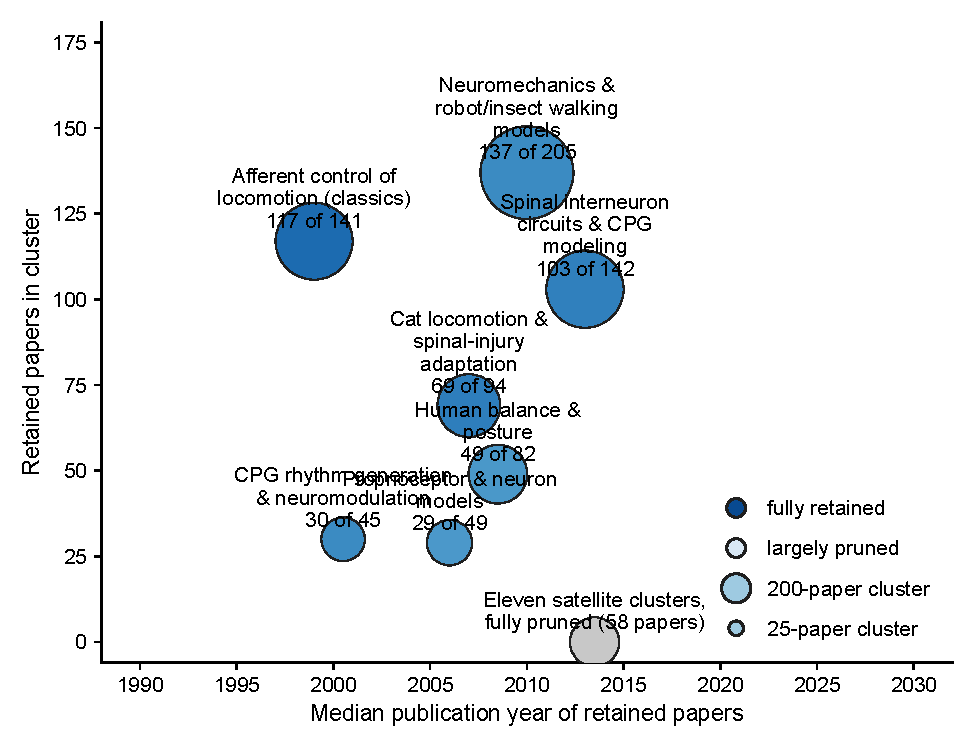
\includegraphics[width=0.92\textwidth]{sadb_clusters.pdf}
\caption[Citation-graph topic clusters of the audited corpus]{The Louvain topic clusters of the audited corpus, one bubble per cluster. Horizontal position is the median publication year of the cluster's retained papers, vertical position the number of retained papers, and bubble area the audited cluster size; darker fill marks a larger retained fraction. The seven clusters with retained papers form the curated core, from the afferent-control classics and spinal-circuit modeling to neuromechanics and robot walking; the gray bubble aggregates the eleven satellite clusters the prune removed in full (58 papers), among them the fish-swimming, flow-and-flight-sensing, and neural-network-method clusters of the prune account. 27 of the 561 retained papers fall outside the citation-graph partition.}
\label{fig:sadb_clusters}
\end{figure}

\section{Curation Methods}\label{sec:sadb_methods}

This section records what a reader needs to know to understand how the corpus was assembled and judged: the sources it came from, the rules a record had to satisfy, the role of the AI tools, and who decided. The reviews this dissertation draws on mark the starting point rather than the method: \citet{van_de_crommert_review_1998} organize the sensory control of the central pattern generator, \citet{windhorst_muscle_2007} assigns functional roles to muscle proprioceptive feedback, and \citet{windhorst_spinal_2022} weighs accumulated spinal-circuit model assumptions against the experimental record. Each synthesizes a slice of the literature; none can be filtered by afferent class, animal preparation, or pathway, none carries its demonstrating papers as attached and followable evidence, and each is fixed at its publication date.

The corpus was assembled from three sources that did not agree: my personal Zotero collection (538 items), the AARL group library's Biology subtree (911 items across 27 collections), and the Airtable base (99 papers). Matching record by record on DOI and normalized title showed that the personal collection was essentially a subset of the group library and that the Airtable base was a small curated subset rather than a mirror, and the gap was imported in verified batches, each written record re-read and checked after writing. The corpus then grew through citation mining, newly saved references, and a bulk pass that imported 372 papers auto-classified from the laboratory's staged PDF collection, bringing the audited corpus to 943 papers, the full set against which every later decision in this chapter was made.

A record's inclusion follows from what the corpus is for: experimental and review literature, and computational models, concerning the afferent control of locomotion and posture and the preparations that establish it. Papers outside that scope, machine-learning and aerodynamics methods papers, flow-sensing work without neurophysiology, and fish swimming biomechanics, were removed in the prune described below, as were duplicates, monographs, and conference abstracts. Within scope, papers for which no text could be found were logged and left bare rather than guessed, and ambiguous cases were flagged for a human ruling rather than decided silently.

The curation was machine-assisted under a division of labor in which the machine drafts and the human rules; the comparative evaluation of the AI tools that motivated this division is reported in Section~\ref{sec:sadb_triage} \citep{bolen_using_2024}. The machine contributed scale: batch drafting from grounded text, automated vocabulary, abstract-paste, and duplicate gates that rejected bad records before anything was written, and per-record verification against the grounding text after the write. I held every decision that required judgment or carried risk: the curation vocabulary and its amendments, the 164 flagged judgment calls, and every single deletion in the prune. Papers for which no text could be found stayed bare by rule rather than guessed, with grounding recovered where the laboratory's own library or a university-authenticated session could provide it.

Pruning then removed 436 records, 382 papers plus 54 orphaned review, model, and pathway records, in three stages: off-topic satellites, duplicates, and orphans first; a rule-built cut list of 290 papers next, ranked by a weighted rubric over citation count, age, rating, network isolation, and record thinness, with 351 protected records (foundational authors, feedback-linked papers, highly cited work, and pre-1940 classics) excluded from consideration; and a final sweep of records whose links the earlier cuts had emptied. The prune was deliberate on two grounds: the working base stood at 1,393 records before the prune, the 943 papers of the audited corpus plus 450 linked review, model, pathway, and recorder records, swollen past the laboratory's free-plan record cap; and a curated resource that answers a design question in ten records beats a haystack of a thousand. No record was destroyed; every deletion was snapshotted, and the packaged explorer carries the 382 cut papers under an archived flag, so the audited corpus remains reconstructible in full.

\section{The Audited Corpus and Curation Coverage}\label{sec:sadb_corpus}

At the close of the curation effort the working base held 957 records: 561 papers, 39 feedback-pathway records, 244 model records, 109 review records, and 4 recorder entries. Coverage of the retained papers is concentrated where the laboratory's design and experimental work needs it. Of the 561 retained papers, 523 carry curation notes, 426 carry animal-preparation tags, 240 carry notes assessing each paper's animal-study potential, 118 are linked to named feedback pathways, 86 carry an afferent classification, and 258 carry notes translating the paper's findings toward robot or simulation use; 550 carry DOIs, and 38 remain bare pending a findable text.

The citation graph was built over the full audited corpus of 943 papers, which includes the 382 records the prune later removed. Within that corpus, 730 papers are connected by 11,130 directed in-corpus citation pairs, and a Louvain community partition of the graph resolves 18 named topic clusters, from the classics of afferent locomotor control and spinal interneuron circuit modeling through human balance and posture to bioinspired flow sensing and deep-learning methods. The partition earned its keep in the prune: the satellite clusters it exposed, the flow-and-flight sensing, fish swimming, and neural-network method clusters, match the topic groups the first prune stage removed. Within that audited corpus, 833 papers carry curation notes and 318 carry attached PDFs. The corpus, its citation graph, its cluster assignments, and the flat corpus export are distributed together in the packaged explorer.

\section{AI-Assisted Literature Triage}\label{sec:sadb_triage}

Expanding a curated corpus is dominated by triage: deciding, paper by paper, what a record is about and whether it belongs. I evaluated AI tools for this task in a comparative study presented at Neuroscience 2024 \citep{bolen_using_2024}. The evaluation found the expected trade: the tools accelerated the population of the database, but their output still required substantial human oversight for accuracy. The curation workflow of Section~\ref{sec:sadb_methods} is the operational answer to that finding. Its gates earned their place on caught failures, including a record that shipped another paper's abstract under its title until the grounding pass flagged it; the human rulings it reserves are the oversight the evaluation showed was necessary, made concrete.

\section{Toward Robot and Simulation Use}\label{sec:sadb_use}

The database exists to feed the sensorium of Chapter~\ref{ch:sns}. Its pathway records enumerate the signal taxonomy the controller's sensory channels implement: Ia afferents carrying length and velocity, Ib afferents carrying force, II afferents carrying length, and contact receptors marking the stance--swing boundary (Section~\ref{sec:preliminary_sim_methods}); Table~\ref{tab:sadb_afferents} summarizes what the corpus establishes for each class. The pathway naming grammar maps directly onto circuit edges, since a record's afferent class fixes the signal encoding, its phase fixes the gating, and its action fixes the sign, so translating a pathway record into a controller connection is a lookup rather than a literature search; Table~\ref{tab:sadb_pathways} lists the principal pathway records with the papers that demonstrate them. The Models table carries the lineage the controller instantiates, from the two-level rhythm-generator and pattern-formation architecture \citep{rybak_modelling_2006} through muscle-reflex walking \citep{geyer_musclereflex_2010} to the two-layer neuromechanical walker the laboratory's controller descends from \citep{deng_neuromechanical_2019}, and the 258 robot-and-simulation translation notes exist precisely to shorten the step from paper to wiring decision. Figure~\ref{fig:sadb_pivot} shows the two-dimension count the explorer's pivotable tables produce over the retained corpus, the afferent classes against the animal preparations: the classical cat preparation carries the largest share of the Ia, Ib, II, and cutaneous records, and the arthropod records enter through the mechanosensory class.

\begin{table}[htbp]
\caption{Afferent classes represented in the Sensory Afferent Database, the signal each class carries, and the pathway roles the corpus records for it. Anchor references are corpus papers linked to the corresponding records; the signal summary for the Ia, II, and Ib rows follows the ensemble afferent recordings of \citet{prochazka_ensemble_1998}.}
\label{tab:sadb_afferents}
\begin{tabularx}{\textwidth}{@{}lllX@{}}
\toprule
\textbf{Class} & \textbf{Receptor} & \textbf{Signal carried} & \textbf{Recorded pathway roles (anchors)} \\
\midrule
Ia & muscle spindle primary & muscle length and velocity & homonymous stretch excitation \citep{eccles_integrative_1958}; reciprocal inhibition of the antagonist pool \citep{jankowska_effect_1967} \\
II & muscle spindle secondary & static muscle length & midlumbar disynaptic relay onto motor nuclei \citep{edgley_interneuronal_1987}; stance-phase support of extensor activity \citep{mazzaro_afferent_2006} \\
Ib & Golgi tendon organ & whole-muscle force & autogenic inhibition at rest, stance-phase reversal to excitation, and the load gate on swing onset \citep{dietz_significance_2000, dominguez_candidate_2020} \\
III/IV & free nerve endings & metabolic and nociceptive signals, converging with cutaneous and group II--III afferents as flexor-reflex afferents & phase-dependent resetting of the locomotor rhythm \citep{schomburg_flexor_1998} \\
Cutaneous & skin and foot-pad receptors & contact and perturbation events & flexor excitation and phase-modulated stance correction \citep{sherrington_flexion_1910, forssberg_stumbling_1979} \\
\bottomrule
\end{tabularx}
\end{table}

\begin{figure}[htbp]
\centering
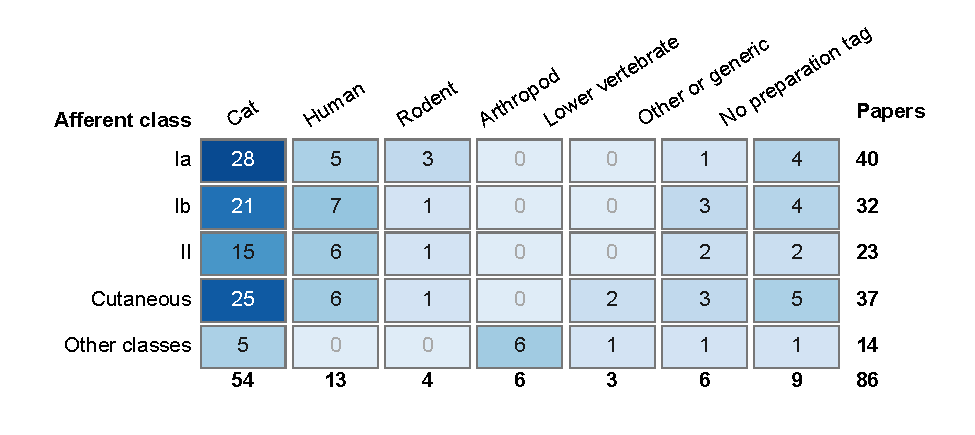
\includegraphics[width=0.96\textwidth]{sadb_pivot.pdf}
\caption[Corpus pivot by afferent class and preparation]{A two-dimension pivot over the retained corpus, of the kind the explorer's pivotable tables produce. Rows are afferent classifications and columns animal preparations; each cell counts the retained papers carrying both tags, so a paper with several preparations or classes counts once in each corresponding cell, and the margins count unique papers. The base is the 86 retained papers that carry an afferent classification, of which 9 have no preparation tag.}
\label{fig:sadb_pivot}
\end{figure}

\begin{sidewaystable}[p]
\caption{Principal feedback-pathway records of the database's Feedback table, named by the fixed grammar of afferent, action, and phase. Linked papers are counted over the full audited corpus of 943 papers; for every pathway listed, the count is unchanged under the retained corpus of 561. Demonstrating references are the corpus papers linked to each record, as curated in the database.}
\label{tab:sadb_pathways}
\fontsize{10pt}{12pt}\selectfont
\begin{tabularx}{\textheight}{@{}llXrp{0.26\textheight}@{}}
\toprule
\textbf{Pathway record} & \textbf{Class} & \textbf{Recorded action in the step cycle} & \textbf{Linked papers} & \textbf{Demonstrating references} \\
\midrule
Ia monosynaptic excitation & Ia & stretch excitation of the homonymous motor pool, with the pathway gain modulated over the step cycle & 7 & \citep{eccles_integrative_1958, capaday_amplitude_1986} \\
Ia reciprocal inhibition & Ia & inhibition of the antagonist motor pool through the Ia inhibitory interneurons, rhythmically active in fictive locomotion & 6 & \citep{jankowska_effect_1967, pratt_ia_1987} \\
Ib disynaptic inhibition & Ib & autogenic non-reciprocal group I inhibition of the loaded muscle's own pool, reduced during stance & 5 & \citep{jankowska_common_1981, stephens_short_1996} \\
Ib disynaptic excitation & Ib & the locomotor reversal: group I input excites synergist extensor pools during the extensor phase, replacing the resting inhibition & 6 & \citep{mccrea_disynaptic_1995, pearson_enhancement_1998} \\
Ib stance to swing & Ib & the load gate: Ib input from ankle extensors prolongs stance, so swing is not initiated while the leg is loaded & 17 & \citep{dietz_significance_2000, dominguez_candidate_2020} \\
Ia or II stance to swing & Ia, II & flexor-length gate on stance termination: lengthening of flexor muscles in late stance ends extension and resets the cycle & 10 & \citep{hiebert_contribution_1996, akay_degradation_2014} \\
type II excitatory & II & stance-phase support of ankle-extensor activity through the midlumbar group II relay & 5 & \citep{edgley_interneuronal_1987, mazzaro_afferent_2006} \\
Cutaneous flexor excitation & Cutaneous & flexion withdrawal and the stumbling corrective reaction, phase-modulated over the cycle & 16 & \citep{sherrington_flexion_1910, forssberg_stumbling_1979} \\
\bottomrule
\end{tabularx}
\end{sidewaystable}

The 39 pathway records extend beyond the mammalian core of Table~\ref{tab:sadb_pathways}: paired excitation and inhibition records cover the chordotonal organs and trochanteral hair plates of insect legs, a load-feedback record covers the campaniform sensilla, and further records hold fictive locomotion without sensory feedback (12 linked papers), group III/IV fatigue, and one paper each for somatosensory, vestibular, and visual contributions to postural control. The controller of Chapter~\ref{ch:sns} implements the mammalian subset. The corpus also reaches ahead to the sensorium extensions planned in Section~\ref{sec:fw_senses}: the human balance and posture cluster and the multisensory recalibration cluster are the entry points for that work, already curated and connected to the locomotor core through the citation graph.

The honest accounting is that the resource is deeper than it is broad in places. The afferent classification covers 86 of 561 retained papers, concentrated in the pathway-rich core rather than spread across the corpus, and the flagged vocabulary gaps (vestibular and visual preparations among them) mark where the classification must grow before the extensions of Section~\ref{sec:fw_senses} can be wired from the database alone. The growth policy follows from the prune: additions should be substantive records or clearly flagged stub twins, never bare rows. The database and the controller of Chapter~\ref{ch:sns} are therefore built as one program: the afferent classes that the controller monitors, the signal encoding each channel carries, and the connection rules its circuit implements all trace to records held here, a mapping Chapter~\ref{ch:sns} documents where the sensory channels are wired.
